\documentclass[a4paper,oneside,12pt]{report}
\setlength\textwidth{145mm}
\setlength\textheight{247mm}
\setlength\oddsidemargin{15mm}
\setlength\evensidemargin{15mm}
\setlength\topmargin{0mm}
\setlength\headsep{0mm}
\setlength\headheight{0mm}
% \openright makes the following text appear on a right-hand page
\let\openright=\clearpage

%% Settings for two-sided (duplex) printing
% \documentclass[12pt,a4paper,twoside,openright]{report}
% \setlength\textwidth{145mm}
% \setlength\textheight{247mm}
% \setlength\oddsidemargin{14.2mm}
% \setlength\evensidemargin{0mm}
% \setlength\topmargin{0mm}
% \setlength\headsep{0mm}
% \setlength\headheight{0mm}
% \let\openright=\cleardoublepage

%% If the thesis has no printed version, symmetric margins look better
% \documentclass[12pt,a4paper]{report}
% \setlength\textwidth{145mm}
% \setlength\textheight{247mm}
% \setlength\oddsidemargin{10mm}
% \setlength\evensidemargin{10mm}
% \setlength\topmargin{0mm}
% \setlength\headsep{0mm}
% \setlength\headheight{0mm}
% \let\openright=\clearpage



\setlength\textwidth{155mm}
\setlength\textheight{247mm}
\setlength\topmargin{-10mm}
% \setlength\headheight{0mm}
\setlength\oddsidemargin{05mm}
\setlength\evensidemargin{05mm}
\let\openright=\clearpage

\renewcommand{\baselinestretch}{1.5}


\usepackage[english]{babel}
\usepackage[T1]{fontenc}
\usepackage[utf8]{inputenc}
\usepackage{lmodern,textcomp}

\usepackage[a-2u]{pdfx}         % metadata v pdf
\usepackage{graphicx}						% vkládání obrázků
\usepackage{caption}						%	popisky
\usepackage{hyperref} 					% odstranění červených okrajů v obsahu
\usepackage{tabularx}           % dynamické tabulkové prostřední
\usepackage{xcolor,colortbl}    % větší barevné množnosti
\usepackage{textpos}            % větší kontrola nad pozicí textu
\usepackage{longtable}          % tabulka s podporou zalamování
\usepackage{fancyhdr}						% možnost stylizovat záhlaví
\usepackage{xurl}								% umožní url zalomit všude
\usepackage{enumitem}           % rozšíření způsobů indexování listu
\usepackage{multicol}           % prostředí pro psaní textu ve sloupcích

%%% Math packages
\usepackage{pgfplots}           % grafy
\usepackage{amsmath}						% rozšíření pro sazbu matematiky
\usepackage{amsthm}							% sazba vět, definic apod.
\usepackage{amssymb} 						% matematické symboly
\usepackage{mathrsfs}  	        % matematické symboly
\usepackage{mathabx}						% matematické symboly
\usepackage{upgreek} 						% pro sazbu řeckých písmen
\usepackage{fixmath}            % zpravuje zápis v matematickém módu dle ISO norem
\usepackage{bbm} 							  % matematické symboly
\usepackage{esint} 						  % další integrály
\usepackage{accents}
\usepackage{arcs}

%%% Bibliography
\usepackage[backend=biber,style=iso-numeric,sortlocale=cs_CZ]{biblatex}  % citace v prostředí biblatex


%%% Basic configuration of packages
\def\columnseprulecolor{\color{black}}
\setlength{\columnseprule}{0.3pt}
\babelprovide[transforms = oneletter.nobreak]{czech}

\hypersetup{pdfborder=0 0 0}
\hypersetup{unicode}
\hypersetup{breaklinks=true}

%%% Configuration of bibliography
\DeclareFieldFormat{labelnumberwidth}{\mkbibbrackets{#1}} % force biblatex to make brackets around numbers
\ExecuteBibliographyOptions{maxcitenames=2} % In citation with full bibliography entry cite just two names at max, per ISO 690
\addbibresource{bibliography.bib}

\let\familynameformat=\textsc % Use caps-and-small-caps for family names in ISO 690 style.

% We want to separate multiple authors in citations by commas
% (while we use semicolons in the bibliography as per the ISO standard)
\DeclareDelimFormat[textcite]{multinamedelim}{\addcomma\space}
\DeclareDelimFormat[textcite]{finalnamedelim}{\space and~}


%%% Please fill in basic information on your thesis, which will be automatically
%%% inserted at the right places. You need to replace ... by real data.

% Type of your thesis:
%	"bc" for Bachelor's
%	"mgr" for Master's
%	"phd" for PhD
%	"rig" for rigorosum
% "sem" for semestral
\def\ThesisType{bc}


\def\ThesisTitle{Surveillance FMCW Radar}

\def\ThesisTitleShort{Surveillance FMCW Radar}

\def\ThesisAuthor{Havránek Kryštof}

\def\MontSubmitted{TODO}

\def\YearSubmitted{2024}

\def\Institution{Czech Technical University in Prague}

\def\Faculty{Faculty of Electrical Engineering}

\def\DepartmentType{Department}

\def\Department{Department of Electromagnetic Field}

\def\Supervisor{Ing. Viktor Adler, Ph.D}

\def\SupervisorsDepartment{Department of Electromagnetic Field}

\def\StudyProgramme{Elektronika a komunikace}

\def\Dedication{%
Dedication.
}

\def\Abstract{%
	TODO
}

% 3 to 5 keywords (recommended) separated by \sep
% Keywords are useful for indexing and searching for the theses by topic.
\def\ThesisKeywords{%
	TODO
}

% If any of your metadata strings contains TeX macros, you need to provide
% a plain-text version for use in XMP metadata embedded in the output PDF file.
% If you are not sure, check the generated thesis.xmpdata file.
\def\AuthorXMP{\ThesisAuthor}
\def\TitleXMP{\ThesisTitle}
\def\KeywordsXMP{\ThesisKeywords}
\def\AbstractXMP{\Abstract}

% If your abstracts are long and do not fit in the infopage, you can make the
% fonts a bit smaller by this setting. (Also, you should try to compress your abstract more.)
\def\InfoPageFont{}
%\def\InfoPageFont{\small}  % uncomment to decrease font size

% If you are studing in a Czech programme, you also need to provide metadata in Czech:
% (in English programmes, this is not used anywhere)

\def\ThesisTitleCS{Přehledový FMCW radar}
\def\DepartmentCS{Katedra elektromagnetického pole}
\def\DepartmentTypeCS{Katedra}
\def\SupervisorsDepartmentCS{Katedra elektromagnetického pole}
\def\StudyProgrammeCS{Elektronika a komunikace}

\def\ThesisKeywordsCS{%
	TODO
}

\def\AbstractCS{%
	TODO
}


%%% This file contains definitions of various useful macros and environments %%%
%%% Please add more macros here instead of cluttering other files with them. %%%

\def\LangCS{cs}
\def\LangEN{en}


%%% Minor tweaks of style

% These macros employ a little dirty trick to convince LaTeX to typeset
% chapter headings sanely, without lots of empty space above them.
% Feel free to ignore.
\makeatletter
\def\@makechapterhead#1{
  {\parindent \z@ \raggedright \normalfont
   \Huge\bfseries \thechapter. #1
   \par\nobreak
   \vskip 20\p@
}}
\def\@makeschapterhead#1{
  {\parindent \z@ \raggedright \normalfont
   \Huge\bfseries #1
   \par\nobreak
   \vskip 20\p@
}}
\makeatother

% make chaptermark non uppercase
\renewcommand{\chaptermark}[1]{%
  \markboth{#1}{}}

% This macro defines a chapter, which is not numbered, but is included in the table of contents.
\def\chapwithtoc#1{
\chapter*{#1}
\addcontentsline{toc}{chapter}{#1}
}

% Slightly less strict rules for placing breaklines inside words
\lefthyphenmin=2
\righthyphenmin=2

% Draw black "slugs" whenever a line overflows, so that we can spot it easily.
% \overfullrule=1mm

% Empty page

\ifx\DocLanguage\LangEN
\newcommand\blankpage{
\newpage
\begin{center}
\vspace*{\fill}
  {Empty page}
\vspace*{\fill}
\end{center}
}

\else
\newcommand\blankpage{
\newpage
\begin{center}
\vspace*{\fill}
  {Prázdná strana}
\vspace*{\fill}
\end{center}
}
\fi


%%% Macros for definitions, theorems, claims, examples, ... (requires amsthm package)
\makeatletter
\def\th@plain{%
  \thm@notefont{}% same as heading font
  \itshape % body font
}
\def\th@definition{%
  \thm@notefont{}% same as heading font
  \normalfont % body font
}
\makeatother

\ifx\DocLanguage\LangEN
\theoremstyle{plain}
\newtheorem{thm}{Theorem}
\newtheorem{lemma}[thm]{Lemma}
\newtheorem{claim}[thm]{Claim}
\newtheorem{defn}{Definition}

\theoremstyle{remark}
\newtheorem*{cor}{Corollary}
\newtheorem*{rem}{Remark}
\newtheorem*{example}{Example}

\else
\theoremstyle{plain}
\newtheorem{thm}{Teorém}
\newtheorem{lemma}[thm]{Lemma}
\newtheorem{claim}[thm]{Tvrzení}
\newtheorem{defn}{Definice}

\theoremstyle{remark}
\newtheorem*{cor}{Důsledek}
\newtheorem*{rem}{Připomínka}
\newtheorem*{example}{Například}

\fi


%%% Tweaks for tables
\newcommand{\pulrad}[1]{\raisebox{1.5ex}[0pt]{#1}}
\newcommand{\mc}[1]{\multicolumn{1}{c}{#1}}
\newcolumntype{C}[1]{>{\centering\arraybackslash}p{#1}}

%%% TODO items
\newcommand{\xxx}[1]{\textcolor{red!}{#1}}


%%% Groups of different numbers, average value
\DeclareMathOperator{\R}{\mathbb{R}}
\DeclareMathOperator{\N}{\mathbb{N}}
\DeclareMathOperator{\Q}{\mathbb{Q}}
\DeclareMathOperator{\C}{\mathbb{C}}
\DeclareMathOperator{\F}{\mathbb{F}}
\DeclareMathOperator{\Z}{\mathbb{Z}}

\DeclareMathOperator{\coord}{\text{coord}}
\DeclareMathOperator{\mgrad}{\text{grad}\,}
\DeclareMathOperator{\mdiv}{\mathrm{div}\,}
\DeclareMathOperator{\mrot}{\mathrm{rot}\,}

%%% Comments inside of mathematical equations, useful for simple substitutions and such
\newcommand{\lcom}{\left\langle\left\langle} %% deprecated
\newcommand{\rcom}{\right\rangle\right\rangle} %% deprecated
\newcommand{\com}[1]{\left\langle\left\langle #1 \right\rangle\right\rangle}

%%% Equals with text over it
\DeclareMathOperator{\eqlh}{\mathrel{\stackrel{\makebox[0pt]{\mbox{\normalfont\tiny L'H}}}{=}}}
\DeclareMathOperator{\eqpp}{\mathrel{\stackrel{\makebox[0pt]{\mbox{\normalfont\tiny PP}}}{=}}}
\newcommand{\eqi}[1]{\mathrel{\stackrel{\makebox[0pt]{\mbox{\normalfont\tiny $#1$}}}{=}}}
\newcommand{\rai}[1]{\mathrel{\stackrel{\makebox[0pt]{\mbox{\normalfont\tiny $#1$}}}{\rightarrow}}}

%% Different lines under text
\newcommand*{\ucheck}[1]{\underaccent{\check}{#1}}
\newcommand*{\uwidecheck}[1]{\underaccent{\widecheck{\hphantom{#1}}}{#1}}
\def\doubleunderline#1{\underline{\underline{#1}}}\makeatletter

%%% Handle " in tikzcd
\newenvironment{tikzcdi}{\shorthandoff{"}\begin{tikzcd}}{\end{tikzcd}\shorthandon{"}}%

%%% Macros for statistics and probability theory
\DeclareMathOperator{\pr}{\textsf{P}}
\DeclareMathOperator{\E}{\textsf{E}\,}
\DeclareMathOperator{\var}{\textrm{var}}
\DeclareMathOperator{\sd}{\textrm{sd}}
\DeclareMathOperator{\ED}{\mathbb{E}}

%%% Other math tweaks
\newcommand{\goto}{\rightarrow}
\newcommand{\gotop}{\stackrel{P}{\longrightarrow}}
\newcommand{\maon}[1]{o(n^{#1})}
\newcommand{\abs}[1]{\left|{#1}\right|}
\ExplSyntaxOn
\NewDocumentCommand{\intd}{m}
{
    \int \clist_map_inline:nn { #1 } { \mathrm{d} ##1 \, }
}
\ExplSyntaxOff % expands \intd{x,y} into \int \mathrm{d}x \mathrm{d}y, used primarily in quantum physics
\newcommand{\isqr}[1]{\frac{1}{\sqrt{#1}}}
\newcommand{\T}[1]{#1^\top}

%% braket notation
\DeclarePairedDelimiter\bra{\langle}{\rvert}
\DeclarePairedDelimiter\ket{\lvert}{\rangle}
\DeclarePairedDelimiterX\braket[2]{\langle}{\rangle}{#1\,\delimsize\vert\,\mathopen{}#2}

%%% Environment with different font size
\newenvironment{localsize}[1]
{%
  \clearpage
  \let\orignewcommand\newcommand
  \let\newcommand\renewcommand
  \makeatletter
  \input{bk#1.clo}%
  \makeatother
  \let\newcommand\orignewcommand
}
{%
  \clearpage
}

%%% Prostředí pro tabulky s centrováním textu v buňce
\newcolumntype{C}[1]{>{\centering\arraybackslash}p{#1}}



%% Titulní strana a různé povinné informační strany
\fancypagestyle{plain}{
  \fancyhf{}
  \renewcommand{\headrulewidth}{0.4pt}
  \renewcommand{\footrulewidth}{0.4pt}
  \fancyhead[C]{}
	\fancyhead[L]{\InstitutionName}
  \fancyhead[R]{\ThesisNameShort}
  \fancyfoot[L]{}
  \fancyfoot[C]{}
  \fancyfoot[R]{\thepage}
}



\begin{document}

%%% TitlePage

\def\TypeBc{bc}
\def\TypeMgr{mgr}
\def\TypePhD{phd}
\def\TypeRig{rig}
\def\TypeSem{sem}

\ifx\ThesisType\TypeBc
\def\ThesisTypeName{bachelor}
\def\ThesisTypeTitle{BACHELOR THESIS}
\fi

\ifx\ThesisType\TypeMgr
\def\ThesisTypeName{master}
\def\ThesisTypeTitle{MASTER THESIS}
\fi

\ifx\ThesisType\TypePhD
\def\ThesisTypeName{doctoral}
\def\ThesisTypeTitle{DOCTORAL THESIS}
\fi

\ifx\ThesisType\TypeRig
\def\ThesisTypeName{rigorosum}
\def\ThesisTypeTitle{RIGOROSUM THESIS}
\fi

\ifx\ThesisType\TypeSem
\def\ThesisTypeName{semestral}
\def\ThesisTypeTitle{SEMESTRAL PROJECT}
\fi

\pagestyle{empty}
\hypersetup{pageanchor=false}

\begin{center}

{\LARGE\bfseries\Institution}

\vspace{-18mm}
\vfill

{\LARGE\Department}

\vfill

\centerline{\mbox{\def\svgwidth{\columnwidth}\scalebox{0.28}{%% Creator: Inkscape 1.1.2 (0a00cf5339, 2022-02-04), www.inkscape.org
%% PDF/EPS/PS + LaTeX output extension by Johan Engelen, 2010
%% Accompanies image file 'logo.pdf' (pdf, eps, ps)
%%
%% To include the image in your LaTeX document, write
%%   \input{<filename>.pdf_tex}
%%  instead of
%%   \includegraphics{<filename>.pdf}
%% To scale the image, write
%%   \def\svgwidth{<desired width>}
%%   \input{<filename>.pdf_tex}
%%  instead of
%%   \includegraphics[width=<desired width>]{<filename>.pdf}
%%
%% Images with a different path to the parent latex file can
%% be accessed with the `import' package (which may need to be
%% installed) using
%%   \usepackage{import}
%% in the preamble, and then including the image with
%%   \import{<path to file>}{<filename>.pdf_tex}
%% Alternatively, one can specify
%%   \graphicspath{{<path to file>/}}
%%
%% For more information, please see info/svg-inkscape on CTAN:
%%   http://tug.ctan.org/tex-archive/info/svg-inkscape
%%
\begingroup%
  \makeatletter%
  \providecommand\color[2][]{%
    \errmessage{(Inkscape) Color is used for the text in Inkscape, but the package 'color.sty' is not loaded}%
    \renewcommand\color[2][]{}%
  }%
  \providecommand\transparent[1]{%
    \errmessage{(Inkscape) Transparency is used (non-zero) for the text in Inkscape, but the package 'transparent.sty' is not loaded}%
    \renewcommand\transparent[1]{}%
  }%
  \providecommand\rotatebox[2]{#2}%
  \newcommand*\fsize{\dimexpr\f@size pt\relax}%
  \newcommand*\lineheight[1]{\fontsize{\fsize}{#1\fsize}\selectfont}%
  \ifx\svgwidth\undefined%
    \setlength{\unitlength}{76.00125bp}%
    \ifx\svgscale\undefined%
      \relax%
    \else%
      \setlength{\unitlength}{\unitlength * \real{\svgscale}}%
    \fi%
  \else%
    \setlength{\unitlength}{\svgwidth}%
  \fi%
  \global\let\svgwidth\undefined%
  \global\let\svgscale\undefined%
  \makeatother%
  \begin{picture}(1,1.0179701)%
    \lineheight{1}%
    \setlength\tabcolsep{0pt}%
    \put(0,0){
\includegraphics[width=\unitlength,page=1]{img/logo.pdf}}%
  \end{picture}%
\endgroup%
}}}

\vspace{-8mm}
\vfill

{\bf\Large \ThesisTypeTitle}

\vfill


\vspace{15mm}

{\LARGE\bfseries\ThesisTitle}


\vfill


{
\centerline{\vbox{\halign{\hbox to 0.45\hsize{\hfil #}&\hskip 0.5em\parbox[t]{0.45\hsize}{\raggedright #}\cr
Supervisor of the \ThesisTypeName{} thesis:&\Supervisor \cr
\ifx\ThesisType\TypeRig\else
\noalign{\vspace{2mm}}
Study programme:&\StudyProgramme \cr
\fi
}}}}

\vspace{15mm}
Prague \MontSubmitted \ \YearSubmitted

\end{center}


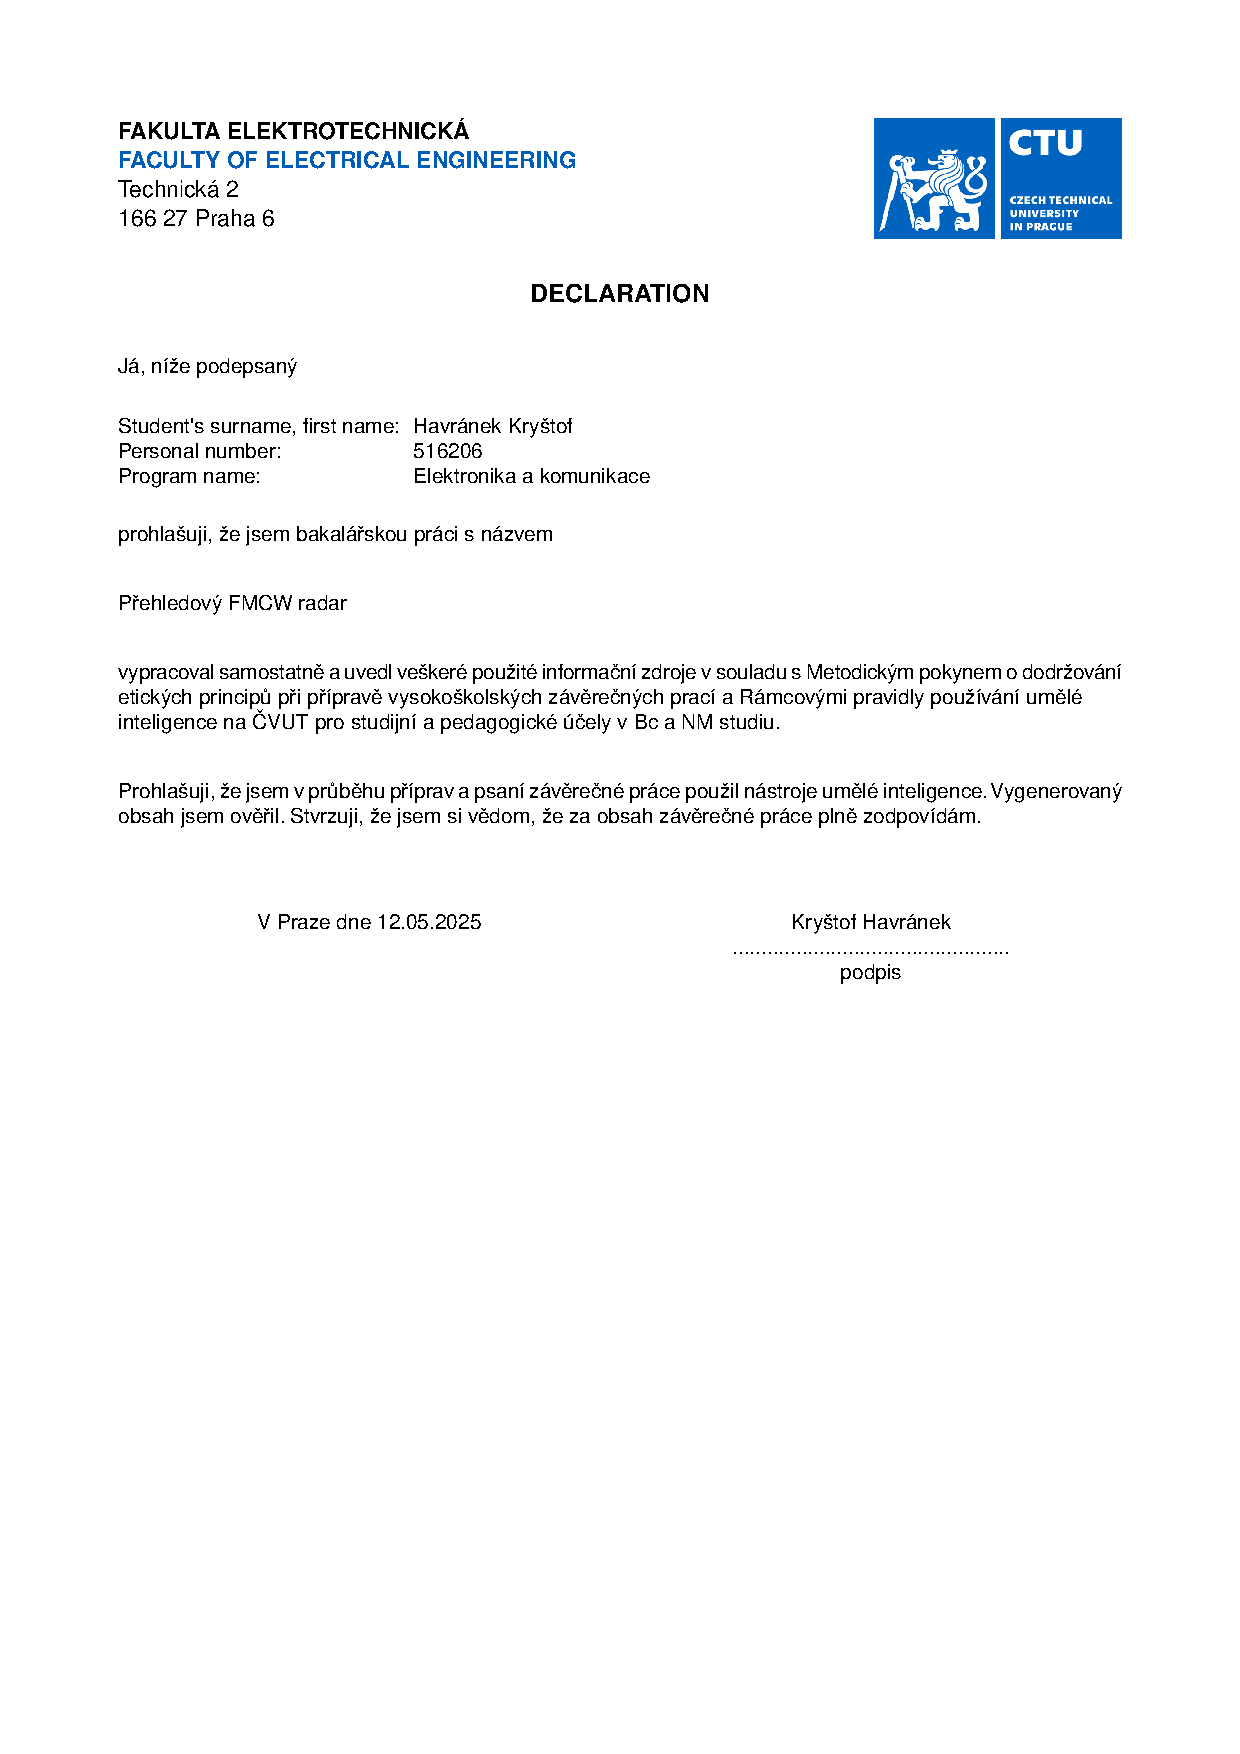
\includepdf{../img/Declaration.pdf}
\newpage
\hypersetup{pageanchor=true}
\protect\pagestyle{plain}
\pagenumbering{roman}


\openright

{\InfoPageFont

\vtop to 0.46\vsize{
\setlength\parindent{0mm}
\setlength\parskip{5mm}

\textbf{Title:} \ThesisTitle \\
\textbf{Author:} \ThesisAuthor \\
\textbf{\DepartmentType:} \Department \\
\textbf{Supervisor:} \Supervisor, \SupervisorsDepartment \\

\textbf{Abstract:}  \Abstract \\

\textbf{Keywords:}
{\def\sep{\unskip, }\ThesisKeywords}

\vfil
}


\vtop to 0.46\vsize{
\setlength\parindent{0mm}
\setlength\parskip{5mm}

\textbf{Název práce:} \ThesisTitleCS \\
\textbf{Autor:} \ThesisAuthor \\
\textbf{\DepartmentTypeCS:} \DepartmentCS \\
\textbf{Vedoucí práce:} \Supervisor, \SupervisorsDepartmentCS \\

\textbf{Abstrakt:} \AbstractCS \\

\textbf{Klíčová slova:}
{\def\sep{\unskip, }\ThesisKeywordsCS}

\vfil
}
}


\newpage

\openright



\tableofcontents

\newpage
\pagenumbering{arabic}
\setcounter{page}{1}


\chapter*{Introduction}
\addcontentsline{toc}{chapter}{Introduction}

The following thesis concerns the realization of a generic surveillance radar system based on FMCW (Frequency-Modulated Continuous Wave) technology.
Conventional FMCW-based surveillance radars often employ multiple receiving antennas or are implemented as MIMO (Multiple-Input Multiple-Output) systems.
In MIMO configurations, electronic beam steering is possible, enabling a larger field of view and the detection of targets in both elevation and azimuth.
Simpler systems, which use only multiple receiving antennas, typically allow for azimuth estimation through phase difference analysis \cite{sandeep2018}.
However, such systems generally require significant processing power and are not capable of providing comprehensive 3D spatial information due to their limited field of view.

To address these limitations, this work proposes a simpler approach: a radar system with just a single RX and TX antenna, where the beam is steered mechanically using a rotary platform.
Initially, the capabilities of the \sirad evaluation board are assessed, followed by the development of a custom two-axis rotary platform.
Both components are then integrated into a unified system, controlled and managed via a MATLAB desktop application.
This integration involves both hardware—namely the rotary platform—and software, including control of the platform and processing of radar data.
Similar systems have been previously developed -- both those relying on a single axis of rotation~\cite{nowok2017, vivet2013} or complex commercial solutions enabling surveillance of the whole 3D space~\cite{blighter}.

FMCW radar operates by transmitting a continuous wave signal whose frequency is modulated over time.
By mixing the transmitted and received signals, harmonic components are produced, with frequencies proportional to the distance of a target \cite{graham2005}.
Applying a Fourier transform to the mixed signal enables the determination of object distances within the scene.
Compared to pulsed radar, FMCW can provide accurate distance measurements with relatively low power consumption \cite{jankiraman2018}.
Velocity estimation is also possible by exploiting the Doppler effect.
However it's nature is more complex than in pulsed systems.


This thesis focuses on the \sirad radar system—a low-cost evaluation board designed to familiarize users with FMCW technology, offering both 24~GHz and 122~GHz headers \cite{siradMAN}.
This versatility allows for a wide range of applications, with detection ranges from a few meters up to 400~meters under ideal conditions \cite{siradMANOld}.
However, due to its relatively low sampling rate and the use of a modest microcontroller, the \sirad is not particularly well-suited for speed measurement: the maximum measurable velocities are well below one meter per second, and even then, measurement accuracy is limited.

To complement the radar, a custom rotary platform was designed and constructed for this thesis.
While commercial solutions exist \cite{standa, carl}, they are often prohibitively expensive and include unnecessary features.
Therefore, a more affordable platform was built from off-the-shelf and 3D-printed components, controlled by an ESP32C6 microcontroller.
This controller interprets G-code-like commands and drives the stepper motors.

Data from both the radar and the platform are processed and visualized within MATLAB.
The processing pipeline follows standard approaches, utilizing techniques such as FFT (Fast Fourier Transform) and CFAR (Constant False Alarm Rate) \cite{richards2022}.
Still, a number of processing steps can be toggled or adjusted by the user, providing considerable flexibility.
Processed data are stored in radar cubes -- a common structure in radar applications \cite{richards2022}; which facilitates the implementation of more advanced post-processing algorithms.
For visualization, the system supports both 2D and 3D representations.

The thesis is organized into five main chapters.
The first provides the theoretical background of FMCW radar technology and its advantages over alternative radar methods.
The second chapter focuses on the \sirad evaluation board, particularly its suitability for surveillance radar applications.
The third chapter describes the design requirements and development process of the custom rotary platform, including its control software.
The fourth chapter gives an overview of the MATLAB desktop application used to control the system and process radar data.
Finally, the fifth chapter delves deeper into the data processing pipeline and available visualization methods.


\chapter{Lorem ipsum}







% vim.ft=tex
\chapter*{Conclusion}
\addcontentsline{toc}{chapter}{Conclusion}

TODO


%%% Bibliography (literature used as a source)
%%%
%%% We employ biblatex to construct the bibliography. It processes
%%% citations in the text (e.g., the \cite{...} macro) and looks up
%%% relevant entries in the bibliography.bib file.
%%%
%%% See also biblatex settings in thesis.tex.

%%% Generate the bibliography. Beware that if you cited no works,
%%% the empty list will be omitted completely.

% We let bibliography items stick out of the right margin a little
\def\bibfont{\hfuzz=2pt}

\printbibliography[heading=bibintoc]

%%% If case you prefer to write the bibliography manually (without biblatex),
%%% you can use the following. Please follow the ISO 690 standard and
%%% citation conventions of your field of research.

% \begin{thebibliography}{99}
%
% \bibitem{lamport94}
%   {\sc Lamport,} Leslie.
%   \emph{\LaTeX: A Document Preparation System}.
%   2nd edition.
%   Massachusetts: Addison Wesley, 1994.
%   ISBN 0-201-52983-1.
%
% \end{thebibliography}


\listoffigures

\listoftables


\openright
\end{document}
